%% ieee_manuscript.tex
%% Latency Optimization in RAG via Edge Computing (Edge-RAG)
%% IEEE conference format. Compiles with tectonic or pdflatex.
\documentclass[conference]{IEEEtran}
\IEEEoverridecommandlockouts

\usepackage{amsmath}
\usepackage{amssymb}
\usepackage{booktabs}
\usepackage{array}
\usepackage{multirow}
\usepackage{tikz}
\usetikzlibrary{positioning,arrows.meta}
\usepackage{pgfplots}
\pgfplotsset{compat=1.18}
\usepackage{url}
\usepackage{cite}
\usepackage[hidelinks]{hyperref}

\newcommand{\code}[1]{\texttt{#1}}

\begin{document}

\title{Latency Optimization in Retrieval-Augmented\\ Generation via Edge Computing:\\ An Analytical Model and Retrieval-Tier Measurements for Edge-RAG}

\author{\IEEEauthorblockN{Mohammad Safari}
\IEEEauthorblockA{Independent Research\\
Email: mo@aioapex.com}}

\maketitle

\begin{abstract}
Retrieval-Augmented Generation (RAG) is the prevailing pattern for grounding large language
models in external knowledge. Its canonical deployment routes every request to a single cloud
region that performs query embedding, vector search and generation, so a geographically distant
user pays a cross-continent round trip before the first token can stream. This paper studies when
relocating the retrieval prefix of RAG to globally distributed edge compute reduces
time-to-first-token (TTFT). We decompose TTFT into four additive terms (network, embedding, search
and generation prefill) and evaluate four deployment topologies with an analytical model: a
centralized region, an edge Worker with an unpooled connection to a central vector database, an
edge Worker with a pooled connection, and an edge Worker with a read replica of the vector tier
near the point of presence. Against a correctly specified centralized baseline, an edge Worker that
still queries a central database gains nothing on the network term; connection pooling is what
makes the edge Worker viable rather than what makes it faster; and the distance-dependent gain, on
the order of one user-to-region round trip, appears only when the vector tier is replicated near
the user. For the retrieval tier we report measurements on PostgreSQL~17 with pgvector~0.8.5 over
300{,}000 768-dimensional vectors: a tuned HNSW index reaches Recall@10 of 0.9999 at a median of
6.7~ms, 1.9 to 2.7 times lower latency than IVFFlat at equal recall, and both indexes are two
orders of magnitude faster than an exact scan. A page-packing model explains why the on-disk HNSW
index size is invariant to the graph degree parameter at this dimensionality, and a corrected
search-cost model is shown to lie below every measured latency. The reference implementation,
simulator, benchmark harness and raw results are released; an end-to-end measurement of the
deployed topologies from multiple geographies is defined as the next step.
\end{abstract}

\begin{IEEEkeywords}
retrieval-augmented generation, edge computing, serverless, V8 isolates, pgvector, HNSW,
approximate nearest neighbor search, connection pooling, time-to-first-token, latency modeling.
\end{IEEEkeywords}

\section{Introduction}

\subsection{Retrieval-augmented generation and the primacy of latency}
Retrieval-Augmented Generation was formalized by Lewis \emph{et al.}~\cite{lewis2020} as the
combination of a parametric memory, a pre-trained sequence-to-sequence generator, with a
non-parametric memory, ``a dense vector index of Wikipedia, accessed with a pre-trained neural
retriever''. The motivation is that parametric-only models' ``ability to access and precisely
manipulate knowledge is still limited, and hence on knowledge-intensive tasks, their performance
lags behind task-specific architectures''~\cite{lewis2020}. The non-parametric component
introduces a retrieval round trip into the request path and is therefore the component most
exposed to where the computation is placed.

For interactive systems that stream tokens, the user-visible latency metric is time-to-first-token
(TTFT): the interval between request submission and the first visible output token. Every stage
that precedes generation (resolving the network path to the service, computing the query
embedding and searching the vector index) is charged in full against TTFT. This work asks under
which conditions moving that retrieval prefix closer to the user reduces TTFT, and by how much.

\subsection{Why centralization is costly}
The default cloud posture concentrates inference and data in a small number of regions. A user
far from that region pays a cross-continent round trip on every interaction. Three effects
compound:
\begin{enumerate}
\item \textbf{Propagation floor.} Light in silica fibre travels at roughly two thirds of its
vacuum speed, about $2.0\times10^{5}$~km/s, or approximately 5~$\mu$s per kilometre one
way~\cite{bozkurt2018}. No engineering removes this term.
\item \textbf{Path inflation.} Deployed fibre does not follow great-circle paths. Bozkurt
\emph{et al.}~\cite{bozkurt2018} measured the ratio of deployed-path latency to the straight-line
fibre ideal across all pairs of the 120 largest U.S. population centres and found a median of 2.1,
reducible to about 1.3 with better use of existing links. That result is scoped to the U.S.
terrestrial backbone; we do not extend it to intercontinental submarine routes
(Section~\ref{sec:net}).
\item \textbf{Connection setup.} Establishing a new PostgreSQL connection over TLS requires, in
Cloudflare's description, ``upwards of seven round-trips (TCP handshake; TLS negotiation; then
auth)'', each of which can take 50 to 200~ms over long distances~\cite{hyperdrive2023}; a later
Cloudflare post gives ``a bare minimum of 5''~\cite{hyperdrive2025}. For a short-lived serverless
invocation that opens a fresh connection per request, this setup cost can exceed the query itself.
\end{enumerate}

\subsection{Contributions}
\begin{enumerate}
\item A four-term additive TTFT model evaluated over four deployment topologies
(Sections~\ref{sec:model}, \ref{sec:net}, \ref{sec:sim}). The model identifies the conditions
under which edge placement helps: pooling is necessary for an edge Worker to match a centralized
baseline, and a near-edge replica of the vector tier is necessary for it to beat one.
\item A corrected cost model for HNSW search in pgvector, in which the candidate-list size and the
corpus size enter additively rather than multiplicatively, validated against our measurements, and
a page-packing model that explains the observed invariance of index size to the graph degree
parameter (Section~\ref{sec:hnsw}).
\item Measurements of the pgvector retrieval tier on 300{,}000 768-dimensional vectors: recall,
latency and throughput for HNSW and IVFFlat across their build and query parameters, with the
artifacts of a memory-constrained host disclosed (Section~\ref{sec:meas}).
\item An open reference implementation (Cloudflare Worker with per-stage \code{Server-Timing}
instrumentation, schema, pooling configuration), the simulator and the benchmark harness, released
so that every figure can be regenerated and the end-to-end measurement defined in
Section~\ref{sec:threats} can be carried out.
\end{enumerate}

\section{Related Work}

\textbf{Retrieval-augmented generation and its latency.} Lewis \emph{et al.}~\cite{lewis2020}
introduced RAG. Subsequent systems work treats retrieval as a first-order latency component of
serving: RAGCache~\cite{ragcache} caches the intermediate states of retrieved knowledge across GPU
and host memory; PipeRAG~\cite{piperag} overlaps retrieval with generation through pipeline
parallelism; TeleRAG~\cite{telerag} prefetches index data from CPU to GPU in parallel with
generation. These works optimize retrieval inside a single serving cluster.
VectorLiteRAG~\cite{vectorlite} shows that, for a 128-million-vector database, CPU-side retrieval
raises TTFT from 197~ms to 606~ms, and the near-memory accelerator of Quinn
\emph{et al.}~\cite{accelrag} reports 13.4 to 27.9 times faster exact search over a 512~GB
database than a server CPU, translating into 1.7 to 26.3 times lower end-to-end inference time.
Those results concern exact search over corpora far larger than ours; we cite them to establish
that retrieval can dominate TTFT at scale, not to transfer their multipliers.

\textbf{Approximate nearest-neighbour search.} HNSW~\cite{malkov2018} builds a multi-layer
proximity graph with links ``separated by their characteristic distance scales''; the authors
report empirically logarithmic scaling of search cost with corpus size. Product
quantization~\cite{jegou2011} and its inverted-file variant established the memory-for-scale
trade underlying IVF-style indexes. ANN-Benchmarks~\cite{annbench} finds that ``very different
approaches to $k$-NN search yield comparable quality-performance trade-offs'', so index choice is
an operating-point decision. pgvector~\cite{pgvector} exposes both an HNSW and an IVFFlat index
inside PostgreSQL.

\textbf{On-device RAG.} EdgeRAG~\cite{edgerag} targets resource-constrained end-user devices and
is evaluated on an NVIDIA Jetson Orin Nano. Its ``edge'' is the device, not a provider's point of
presence; we cite it for two phenomena relevant here, the memory footprint of dense indexes (an
18.5~GB index for 5.23 million FEVER records) and embedding-generation tail latency (most clusters
under 500~ms, some over 2~s; an IVF baseline whose 95th-percentile retrieval latency exceeds the
median by over 64 times on Natural Questions).

\textbf{Serverless execution and cold starts.} Cloudflare states that its V8-isolate runtime loads
a Worker in about 5~ms~\cite{cfcoldstart}; Python Workers, which carry an interpreter, start in
about 1~s with memory snapshots~\cite{cfpython}. Cloudflare's container product documents cold
starts ``often in the 1--3 second range''~\cite{cfcontainers}; a third-party benchmark of 700 boots
reports medians of 1.7 to 10.5~s, 95th percentiles of 15.6 to 24.4~s and a maximum of 58.6~s across
four workloads~\cite{alchemy2026}. Dirigent~\cite{dirigent} shows that sandbox initialization of
``10--100s of milliseconds'' is dwarfed by cluster scheduling latency in real FaaS deployments. All
cold-start figures used here are either vendor-reported or single-benchmark; we treat them as
order-of-magnitude evidence only.

\textbf{Edge RAG on managed platforms.} Cloudflare's own tutorial~\cite{cfragtutorial} builds RAG
from Workers AI (the \code{bge-base-en-v1.5} embedding model) and Vectorize, which the vendor
describes as ``a globally distributed vector database''~\cite{cfvectorize}. That stack is the
vendor default for the problem studied here. This paper instead pairs the edge Worker with a
self-managed PostgreSQL and pgvector tier through a connection pool, because it allows the vector
tier to be shared with an existing relational schema and because pgvector's index internals are
open and measurable. A direct comparison against Vectorize is part of the measurement plan in
Section~\ref{sec:threats}.

\textbf{Fibre-infrastructure latency.} Bozkurt \emph{et al.}~\cite{bozkurt2018} provide the
route-inflation measurement used in Section~\ref{sec:net}.

\section{System Architecture}

\subsection{Reference topologies}
We consider a user at great-circle distance $D$ from the central cloud region that hosts the
vector tier, and a nearby point of presence (PoP) at distance $d_{\mathrm{edge}} \ll D$
(Fig.~\ref{fig:topo}). In the centralized baseline every stage is charged the full user-to-region
path once; the database is in the same region as the application, so connection setup, if not
pooled, costs seven in-region round trips of about a millisecond each. In the three Edge-RAG
variants the Worker embeds the query inside the PoP, removing the in-region embedding hop, and
reaches the vector tier either with a fresh connection per request (edge-unpooled), through a warm
pool (edge-pooled), or through a pool to a replica near the PoP (edge-replica). Generation may
remain central in all variants; it is outside the scope of this study.

\begin{figure}[t]
\centering
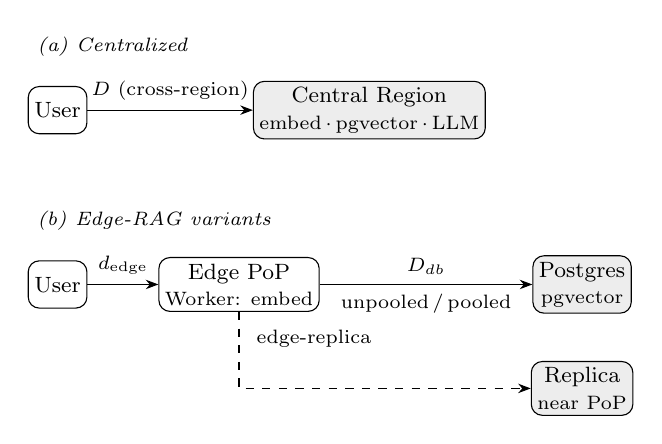
\begin{tikzpicture}[font=\footnotesize,>={Stealth[length=1.6mm]},
  box/.style={draw,rounded corners,align=center,inner sep=2.2pt,minimum height=6mm},
  reg/.style={box,fill=black!7}]
\node[box] (u1) {User};
\node[reg,right=21mm of u1] (c1) {Central Region\\{\scriptsize embed\,$\cdot$\,pgvector\,$\cdot$\,LLM}};
\draw[->] (u1) -- node[above,font=\scriptsize]{$D$ (cross-region)} (c1);
\node[font=\scriptsize\itshape,anchor=west] at ([yshift=5mm]u1.north west) {(a) Centralized};
\node[box,below=16mm of u1] (u2) {User};
\node[box,right=9mm of u2] (e2) {Edge PoP\\{\scriptsize Worker: embed}};
\node[reg,right=27mm of e2] (d2) {Postgres\\{\scriptsize pgvector}};
\node[reg,below=6mm of d2] (r2) {Replica\\{\scriptsize near PoP}};
\draw[->] (u2) -- node[above,font=\scriptsize]{$d_{\mathrm{edge}}$} (e2);
\draw[->] (e2) -- node[above,font=\scriptsize]{$D_{db}$} node[below,font=\scriptsize]{unpooled\,/\,pooled} (d2);
\draw[->,dashed] (e2.south) |- (r2.west);
\node[font=\scriptsize,anchor=north west] at ([xshift=1mm,yshift=-1mm]e2.south) {edge-replica};
\node[font=\scriptsize\itshape,anchor=west] at ([yshift=5mm]u2.north west) {(b) Edge-RAG variants};
\end{tikzpicture}
\caption{Centralized baseline and the three Edge-RAG variants. The Worker embeds within the PoP
and reaches the vector tier with a fresh connection per request, a pooled connection, or a pooled
connection to a near-PoP replica.}
\label{fig:topo}
\end{figure}

\subsection{Isolates versus containers for per-request edge execution}
Per-request execution in hundreds of locations without a warm pool everywhere is the workload
where the start-up cost of the execution unit dominates. Containers and microVMs construct an
image, a runtime and an application before serving; the vendor's own figure for its container
product is 1 to 3~s~\cite{cfcontainers} and third-party measurements show a long
tail~\cite{alchemy2026}. V8 isolates run many tenants' code as sandboxed contexts inside one
already-running process, so there is no per-request OS or runtime boot; the vendor states about
5~ms to load a JavaScript Worker~\cite{cfcoldstart}. For a retrieval prefix that runs for tens of
milliseconds, a multi-second start would exceed the work itself. Two caveats apply. The 5~ms figure
is vendor-reported and JavaScript-only; Python Workers start in about 1~s~\cite{cfpython}. And we
do not make a specific claim about Firecracker snapshot-restore times, which vary by workload and
measurement~\cite{alchemy2026}.

\subsection{Edge embedding}
The query embedding precedes search and is therefore on the critical path. The reference
implementation uses Workers AI, whose \code{@cf/baai/bge-base-en-v1.5} model produces
768-dimensional vectors with a 512-token input limit~\cite{bge}. Small encoders compiled to
WebAssembly can run inside the isolate itself. EdgeRAG's on-device results~\cite{edgerag} show
that embedding-generation tail latency can be severe; the design consequence for Edge-RAG is to
keep the encoder small and warm and to measure the tail, which the Worker's per-stage timing header
enables.

\subsection{Retrieval tier}
The retrieval tier is PostgreSQL with pgvector. Vectors are stored in a \code{vector(768)} column;
cosine distance uses the \code{<=>} operator. HNSW (graph,~\cite{malkov2018}) offers the highest
query-time recall per unit latency at a memory and build-time cost; IVFFlat (inverted lists, the
IVF half of~\cite{jegou2011}) builds faster and its recall is controlled by the number of lists
probed. Section~\ref{sec:meas} measures both.

\subsection{Connection pooling}
A serverless invocation must not open a fresh database connection per request. Cloudflare
Hyperdrive ``maintains a pool of connections to your database. These are optimally placed to
minimize the latency for your applications''~\cite{hyperdrivedocs}; PgBouncer in transaction mode
is the self-managed equivalent. Pooling removes the connection-setup round trips on the
PoP-to-origin leg. It does not remove the propagation distance between PoP and origin, which each
query still crosses once (Section~\ref{sec:sim}).

\section{Implementation}
The accompanying files are \code{worker.ts}, \code{wrangler.toml}, \code{package.json},
\code{schema.sql}, \code{hyperdrive.md}, \code{latency\_sim.py}, \code{bench.py},
\code{docker-compose.yml} and \code{results/}.

\subsection{Cloudflare Worker}
The Worker validates the request, embeds the query through the Workers AI binding, runs a cosine
ANN query over the Hyperdrive-pooled connection, and returns the top-$k$ context together with a
\code{Server-Timing} header carrying the measured duration of the embedding stage, the search
stage and the whole invocation. Two implementation details matter for correctness. First,
\code{SET LOCAL hnsw.ef\_search} only takes effect inside a transaction block; outside one
PostgreSQL emits a warning and ignores it, and under a transaction-mode pooler the \code{SET} and
the \code{SELECT} may not share a server connection. The Worker therefore issues both inside a
single \code{sql.begin(...)} transaction. Second, named prepared statements are disabled because
they are not safe under transaction pooling. The Worker type-checks against
\code{@cloudflare/workers-types}; it has not yet been deployed and measured, which is the subject
of Section~\ref{sec:threats}.

\subsection{Schema and index parameters}
\code{schema.sql} defines the \code{documents} table with \code{embedding vector(768)}, 3{,}072
bytes of raw vector per row. If vectors are L2-normalized at write time, cosine distance equals
one minus the dot product and \code{vector\_cosine\_ops} is the appropriate operator class. The
HNSW parameters follow the pgvector documentation~\cite{pgvector}: \code{m} (default 16) bounds the
number of links per node; \code{ef\_construction} (default 64) is the candidate-list size at build
time; \code{hnsw.ef\_search} (default 40) is the candidate-list size at query time and is the
principal run-time recall dial. For IVFFlat, \code{lists} is set at build time and
\code{ivfflat.probes} at query time. Tables~\ref{tab:hnsw} and~\ref{tab:ivf} quantify the effect
of each dial on our corpus.

\subsection{Pooling configuration}
\code{hyperdrive.md} gives the Hyperdrive binding and an equivalent \code{pgbouncer.ini} in
transaction mode. The Worker reads \code{env.HYPERDRIVE.connectionString}, so the driver connects
to a local pooled endpoint rather than to the origin.

\subsection{Observations from building the benchmark harness}
\begin{itemize}
\item \textbf{Ingestion was bound by client-side serialization.} Loading 300{,}000 rows through a
text \code{COPY FROM STDIN} took 631~s, about 28{,}500 rows per minute, with the time spent
formatting floats in Python. A binary \code{COPY} using pgvector's wire format (\code{int16}
dimension, \code{int16} unused, then big-endian \code{float4} values) from a NumPy buffer avoids
per-element string conversion; the harness keeps text \code{COPY} for portability.
\item \textbf{Parallel index builds need shared memory.} pgvector's parallel HNSW build allocates a
dynamic shared-memory segment; on a container with a 1~GB \code{/dev/shm}, the 300{,}000-vector
build requested 1.25~GB and aborted. Building serially
(\code{max\_parallel\_maintenance\_workers = 0}) uses backend-local \code{maintenance\_work\_mem}
instead, at the cost of build time.
\item \textbf{IVFFlat build memory scales with \code{lists}.} A \code{lists = 4000} build required
3{,}738~MB of \code{maintenance\_work\_mem} against a 2{,}048~MB budget and failed. On constrained
hosts the build step, not the query, can be the binding limit.
\end{itemize}

\section{Model and Evaluation}

\subsection{Additive TTFT model}\label{sec:model}
We model the latency to first useful output as
\begin{equation}
T_{\mathrm{total}} = T_{\mathrm{network}} + T_{\mathrm{embed}} + T_{\mathrm{search}} + T_{\mathrm{generation}},
\label{eq:total}
\end{equation}
where for streaming interfaces $T_{\mathrm{generation}}$ is the generator's prefill time to its
first token. $T_{\mathrm{network}}$ collects all propagation and protocol round trips on the
request path before generation; $T_{\mathrm{embed}}$ is embedding compute plus any hop to reach the
embedder; $T_{\mathrm{search}}$ is index traversal plus, if the connection is not pooled,
connection acquisition. Edge placement can change $T_{\mathrm{network}}$ and the hop component of
$T_{\mathrm{embed}}$; it does not change search compute or generation unless those are also
relocated. $T_{\mathrm{generation}}$ is held fixed across topologies throughout.

\subsection{Network model}\label{sec:net}
Let $c_f \approx 2.0\times10^{5}$~km/s. For straight-line distance $D$ and route-inflation factor
$\rho$,
\begin{equation}
\mathrm{RTT}(D) = \frac{2\rho D}{c_f}.
\label{eq:rtt}
\end{equation}
For U.S. terrestrial scenarios we use the measured median $\rho = 2.1$~\cite{bozkurt2018}. For
intercontinental scenarios that traverse submarine cables, the U.S. backbone median does not
apply; the simulator uses $\rho = 1.3$ as an explicitly labelled assumption and accepts a measured
round-trip time per scenario in its place. With that assumption, Sydney to Ashburn (15{,}900~km)
models at 207~ms; with the U.S. factor it would model at 334~ms, well above the 50 to 200~ms per
round trip cited by the vendor for long paths~\cite{hyperdrive2023}. The measured value will
replace the assumption in the next phase of this work.

Connection setup adds $T_{\mathrm{setup}} \approx n_{rt}\,\mathrm{RTT}(D_{db})$ with
$n_{rt} \approx 7$~\cite{hyperdrive2023} on the leg between the connecting party and the database.
For the centralized topology that leg is in-region and $T_{\mathrm{setup}}$ is a few milliseconds;
for an unpooled edge Worker it spans $D_{db}$ and pooling reduces it to zero at steady state.

\subsection{HNSW search cost and index size}\label{sec:hnsw}
\textbf{Search cost.} The candidate-list-bounded beam search of HNSW runs only at layer 0, where
each element has up to $2m$ links; the upper layers are a greedy descent with a candidate list of
one over about $\log N$ levels. The number of distance evaluations per query is therefore additive
in the two terms:
\begin{equation}
N_{\mathrm{dist}} \approx c\,\mathrm{ef}\,(2m) + m\log_2 N,
\label{eq:ndist}
\end{equation}
with $c$ a constant below one that accounts for neighbours already in the visited set ($c = 0.5$
in the simulator). An earlier draft of this work used a multiplicative form
$c\,\mathrm{ef}\,\bar m \log N$; that form predicts a bandwidth floor of 44.7~ms for the
configuration that we measured at 6.7~ms and is withdrawn. Each evaluation over $d$-dimensional
single-precision vectors reads $4d$ bytes and performs about $2d$ floating-point operations; for
$d = 768$ that is 3{,}072 bytes and about 1{,}536 operations. Because traversal is random access
over the graph, bytes moved per query,
\begin{equation}
B_{\mathrm{query}} \approx 4d\,N_{\mathrm{dist}},
\label{eq:bytes}
\end{equation}
divided by an effective random-access bandwidth gives a lower bound on search compute. The
simulator's \code{--validate} mode checks this bound against every HNSW row of our measurements:
with $c = 0.5$ and an assumed 8~GB/s, the bound ranges from 0.36~ms to 5.14~ms and lies below the
measured median in all twelve configurations, at 1 to 59 percent of it. The bound is consistent
with the data; it is not a fitted predictor.

\textbf{Index size.} pgvector stores each element's vector and its neighbour list in 8~KiB heap
pages, and tuples are not split across pages. With $d = 768$, an element tuple is about 3{,}104
bytes and a neighbour tuple about $6(2m + m/(m-1)) + 8$ bytes, so exactly two
element-plus-neighbour pairs fit in a page for every $m$ up to about 48. The index therefore
occupies $\lceil N/2 \rceil$ pages regardless of $m$: for $N = 300{,}000$ that is 150{,}000 pages,
or 1{,}171.9~MiB, which is the size PostgreSQL reported for both the $m = 16$ and the $m = 32$
index (Table~\ref{tab:hnsw}). The practical consequence is that raising $m$ costs build time and
query bandwidth at this dimensionality, not disk or buffer-cache footprint. For capacity planning,
raw vectors alone are $4dN$ bytes, 2.86~GiB per million 768-dimensional vectors, and the working
set must remain in memory for the random-access traversal to stay in the millisecond range.

\subsection{Simulation results}\label{sec:sim}
\code{latency\_sim.py} evaluates the four topologies of Fig.~\ref{fig:topo} with the constants
above, an embedding time of 25~ms in either location, a 3~ms in-region hop to a separate embedding
service in the centralized case, the measured 6.7~ms search median from Section~\ref{sec:meas},
and a fixed 400~ms generation prefill. It performs no network I/O and every input is labelled by
source in the script. Table~\ref{tab:sim} gives the network term and TTFT for the trans-Pacific
scenario; the other scenarios follow the same pattern with smaller magnitudes.

\begin{table}[t]
\caption{Modelled TTFT for a Sydney user with the vector tier in Ashburn ($\rho = 1.3$ assumed,
RTT 207~ms; $T_{\mathrm{generation}} = 400$~ms fixed).}
\label{tab:sim}
\centering
\begin{tabular}{@{}l r r r@{}}
\toprule
Topology & $T_{\mathrm{network}}$ (ms) & TTFT (ms) & vs.\ centralized \\
\midrule
centralized   & 206.7   & 641.4   & \\
edge-unpooled & 1{,}654.1 & 2{,}085.8 & $+1{,}444.4$ \\
edge-pooled   & 207.2   & 638.9   & $-2.5$ \\
edge-replica  & 1.1     & 432.8   & $-208.6$ \\
\bottomrule
\end{tabular}
\end{table}

Three conclusions follow, and they hold at every distance in the sweep.
\begin{enumerate}
\item An edge Worker with a fresh connection per request is far worse than the centralized
baseline: seven setup round trips over the PoP-to-database distance are charged on every request.
Pooling removes 1{,}447~ms in this scenario and is what makes an edge Worker viable at all.
\item An edge Worker with a pooled connection to a central vector tier matches the centralized
baseline to within the assumed 3~ms embedding hop. The user's request still crosses the same
distance once, now between the PoP and the database instead of between the user and the region.
Relocating compute while leaving the data central yields no network benefit.
\item The distance-dependent gain appears only when the vector tier is replicated near the PoP:
208.6~ms at Sydney, 78.6~ms at London, 75.5~ms for a U.S. coast-to-coast user, and under 10~ms
within a metropolitan area. Its magnitude is one user-to-region round trip, and it comes with the
replication-lag and consistency questions listed in Section~\ref{sec:threats}.
\end{enumerate}
Under the model, generation at 400~ms remains the largest single term in every topology; the
edge-replica variant reduces TTFT for a trans-Pacific user by about one third, not by an order of
magnitude.

\subsection{Retrieval-tier measurements}\label{sec:meas}
\textbf{Setup.} PostgreSQL 17.10 with pgvector 0.8.5 in a Docker VM limited to 4.8~GiB of memory
on an 8-core, 8~GB laptop-class host. The corpus is 300{,}000 L2-normalized 768-dimensional vectors
drawn from a mixture of 1{,}000 Gaussians, generated by \code{bench.py} with a fixed seed. Ground
truth is the exact top-10 by brute-force cosine over the full corpus. Recall@10 is measured for
1{,}000 held-out queries drawn from the same mixture; the exact-scan baseline used the first 30 of
them. Queries are issued serially over one connection, so the reported throughput is a lower
bound. The index path is forced with \code{enable\_seqscan = off} and confirmed with
\code{EXPLAIN}. The exact invocation, server versions and known artifacts are recorded by the
harness in \code{results/summary.json} and in \code{results/ERRATA.md}.

This run had no warm-up pass and a single timed sweep per configuration, with \code{ef\_search}
swept in ascending order after each build; the harness now performs a warm-up and three repeats,
and the rerun on server-class hardware is planned. The consequences for the latency columns are
discussed in Section~\ref{sec:threats}. The recall columns are unaffected by caching.

\begin{table*}[t]
\caption{HNSW on 300{,}000 $\times$ 768 vectors: Recall@10, latency and serial throughput versus
\code{ef\_search}. Index size 1172~MB for every build.}
\label{tab:hnsw}
\centering
\begin{tabular}{@{}c c c c c c c c@{}}
\toprule
Build ($m$ / ef\_c) & Build (s) & \code{ef\_search} & Recall@10 & p50 (ms) & p95 (ms) & p99 (ms) & QPS (serial) \\
\midrule
\multirow{4}{*}{16 / 64} & \multirow{4}{*}{293.9} & 40  & 0.903 & 12.50 & 42.45 & 72.41  & 60.1 \\
                         &                        & 100 & 0.933 & 8.07  & 35.63 & 110.16 & 77.6 \\
                         &                        & 200 & 0.952 & 3.92  & 7.42  & 11.26  & 228.3 \\
                         &                        & 400 & 0.973 & 8.03  & 25.74 & 51.12  & 96.0 \\
\cmidrule(lr){1-8}
\multirow{4}{*}{16 / 200} & \multirow{4}{*}{669.4} & 40  & 0.972 & 25.71 & 114.27 & 217.55 & 27.4 \\
                          &                        & 100 & 0.998 & 12.28 & 30.40  & 55.85  & 70.3 \\
                          &                        & 200 & 0.9999 & 9.43 & 40.84 & 83.95 & 70.3 \\
                          &                        & 400 & 0.9999 & 6.70 & 18.72 & 35.70 & 116.7 \\
\cmidrule(lr){1-8}
\multirow{4}{*}{32 / 200} & \multirow{4}{*}{n/a\textsuperscript{\dag}} & 40  & 0.996 & 21.93 & 79.94 & 162.82 & 33.9 \\
                          &                        & 100 & 0.999 & 7.98  & 24.63 & 57.70 & 97.5 \\
                          &                        & 200 & 0.999 & 6.29  & 12.26 & 23.97 & 146.5 \\
                          &                        & 400 & 0.9998 & 8.71 & 24.94 & 43.32 & 90.8 \\
\bottomrule
\end{tabular}

\vspace{2pt}
{\footnotesize \textsuperscript{\dag}The host suspended overnight during this build; the recorded
wall-clock includes system sleep and is not reported. The query rows for this build ran after wake
and are valid.}
\end{table*}

\begin{table}[t]
\caption{IVFFlat (\code{lists = 1000}; build 166.7~s; index 1178~MB): Recall@10 and latency
versus \code{probes}.}
\label{tab:ivf}
\centering
\footnotesize
\begin{tabular}{@{}c c c c c c@{}}
\toprule
\code{probes} & Recall@10 & p50 (ms) & p95 (ms) & p99 (ms) & QPS \\
\midrule
1   & 0.873  & 9.55  & 29.20  & 55.82  & 77.6 \\
10  & 0.9999 & 18.08 & 39.95  & 94.43  & 45.3 \\
40  & 0.9999 & 41.63 & 75.24  & 97.17  & 22.7 \\
100 & 0.9999 & 75.33 & 164.22 & 208.94 & 11.7 \\
\bottomrule
\end{tabular}
\end{table}

\begin{figure}[t]
\centering
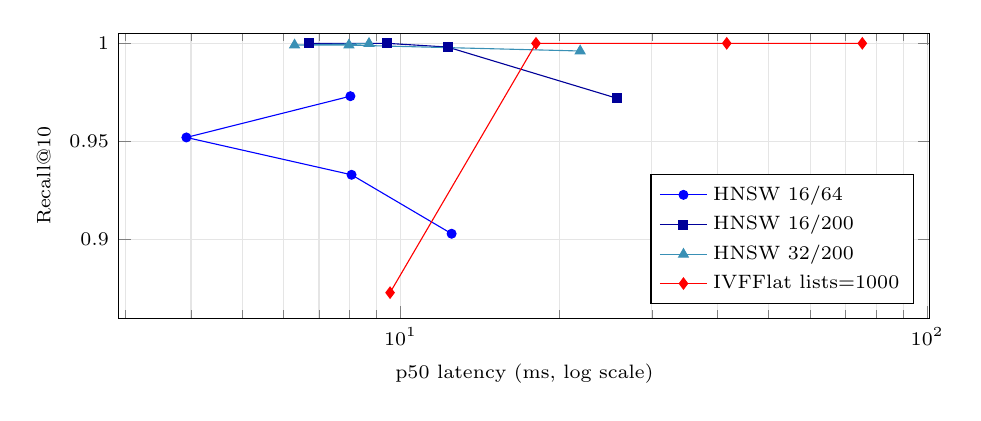
\begin{tikzpicture}
\begin{axis}[width=0.98\columnwidth,height=5.2cm,
  xlabel={p50 latency (ms, log scale)}, ylabel={Recall@10}, xmode=log,
  ymin=0.86, ymax=1.005, grid=both, grid style={black!10},
  legend style={font=\scriptsize, at={(0.98,0.05)}, anchor=south east, cells={anchor=west}},
  tick label style={font=\scriptsize}, label style={font=\scriptsize}]
\addplot[mark=*, mark size=1.6pt, blue]  coordinates {(12.50,0.903) (8.07,0.933) (3.92,0.952) (8.03,0.973)};
\addlegendentry{HNSW 16/64}
\addplot[mark=square*, mark size=1.6pt, blue!60!black] coordinates {(25.71,0.972) (12.28,0.998) (9.43,0.9999) (6.70,0.9999)};
\addlegendentry{HNSW 16/200}
\addplot[mark=triangle*, mark size=2pt, cyan!70!black] coordinates {(21.93,0.996) (7.98,0.999) (6.29,0.999) (8.71,0.9998)};
\addlegendentry{HNSW 32/200}
\addplot[mark=diamond*, mark size=2pt, red] coordinates {(9.55,0.873) (18.08,0.9999) (41.63,0.9999) (75.33,0.9999)};
\addlegendentry{IVFFlat lists=1000}
\end{axis}
\end{tikzpicture}
\caption{Recall@10 versus median latency for every configuration in Tables~\ref{tab:hnsw}
and~\ref{tab:ivf}. Points within a series are in ascending order of the query-time dial; the
non-monotone latency inside each HNSW series reflects cache warming in this single-sweep run
(Section~\ref{sec:threats}).}
\label{fig:pareto}
\end{figure}

A second IVFFlat build with \code{lists = 4000} failed for lack of \code{maintenance\_work\_mem}
(Section~IV-D). An exact sequential scan over the corpus, the brute-force baseline, measured
Recall@10 of 1.000 at a median of 1{,}061.6~ms over 30 queries. Fig.~\ref{fig:pareto} plots every
configuration.

\textbf{Findings.}
\begin{enumerate}
\item Recall rises with \code{ef\_search} within every build and with \code{ef\_construction} and
$m$ across builds. At \code{ef\_search = 40} the recall floor is 0.903, 0.972 and 0.996 for the
three builds; the single exception to monotonicity is at \code{ef\_search = 400}, where the
$m = 32$ build scores 0.9998 against 0.9999 for $m = 16$, a difference of one neighbour in ten
thousand.
\item At Recall@10 of 0.9999, HNSW serves at a median of 6.70, 8.71 or 9.43~ms depending on the
build, against 18.08~ms for IVFFlat with \code{probes = 10}: 1.9 to 2.7 times lower latency and
1.6 to 2.6 times higher serial throughput. We report the range rather than the best ratio because
the median varies by up to 3.2 times between sweeps of the same build
(Section~\ref{sec:threats}).
\item At Recall@10 of at least 0.99, HNSW medians range from 6.3 to 21.9~ms, 48 to 169 times
faster than the exact scan; at 0.95 recall the fastest configuration reaches 3.9~ms, 271 times
faster. Both index families place retrieval in the millisecond range that the model of
Section~\ref{sec:sim} assumes.
\item IVFFlat recall saturates by \code{probes = 10}; raising \code{probes} to 40 and 100
multiplies the median latency by 2.3 and 4.2 with no recall gain.
\item Build cost is asymmetric: IVFFlat built in 166.7~s, HNSW in 293.9~s at
\code{ef\_construction = 64} and 669.4~s at 200, with the $m = 32$ build time unavailable.
\item Index size is invariant to $m$ at this dimensionality, as the page-packing model of
Section~\ref{sec:hnsw} predicts.
\end{enumerate}

\section{Discussion}
The model and the measurements support a narrower claim than ``edge RAG is faster''. The retrieval
prefix is placement-bound, but the placement that matters is that of the data, not of the compute.
An edge Worker with a pooled connection to a central vector tier is neither better nor worse than
a centralized deployment on the network term; it becomes better only when the vector tier has a
replica near the PoP, and then by about one user-to-region round trip, which for trans-Pacific
users is on the order of 200~ms out of a modelled TTFT of 640~ms. Connection pooling is a
precondition for the edge Worker rather than an advantage over the baseline. Generation remains the
largest term everywhere.

Two properties of the platform are what make the edge-replica topology practical. Isolate start-up
in milliseconds allows per-request execution in many locations without warm pools; and a pool
placed between the Worker and the database removes the setup round trips that would otherwise make
an edge Worker slower than the centralized baseline by more than a second. Neither property is a
contribution of this paper; the contribution is to quantify which combination of them yields a
gain, and the conditions under which it does not.

On the retrieval tier, the measurements confirm that a tuned HNSW index in pgvector serves at
single-digit-to-low-tens-of-millisecond medians at recall above 0.99 for a corpus of this size,
and that the query-time dial \code{ef\_search}, not the build parameters, is the appropriate
control for the recall-latency operating point. The page-packing result implies that, for
768-dimensional vectors, increasing $m$ is free in storage but not in build time or per-query
bandwidth.

\section{Threats to Validity, Limitations and Future Work}\label{sec:threats}

\subsection{Internal validity}
\begin{itemize}
\item \textbf{Latency noise in Table~\ref{tab:hnsw}.} Without a warm-up pass, the first sweeps
after each build include cold-cache page reads, and 99th-percentile values rest on ten
observations. Within the $m = 16$, \code{ef\_construction = 64} build the median falls from 12.50
to 3.92~ms and then rises to 8.03~ms across the four ascending sweeps, a pattern that reflects
cache warming, not the dial. Ratios between configurations should be read with this 3.2-times band
in mind; the recall columns are unaffected.
\item \textbf{Ground truth precision.} The corpus was written to PostgreSQL with six significant
figures; ground truth was computed from full-precision floats. Near-ties may flip at the fourth
decimal of recall.
\item \textbf{Single host, single run.} No confidence intervals are reported. The harness now
supports warm-up and repeats.
\end{itemize}

\subsection{External validity}
\begin{itemize}
\item \textbf{Synthetic vectors.} Gaussian mixtures do not reproduce the intrinsic dimensionality
of text embeddings; recall at a given \code{ef\_search} will differ on real corpora.
\item \textbf{Scale and hardware.} 300{,}000 vectors on a 4.8~GiB VM. Server-class memory and
corpora of millions of vectors will change absolute latencies and may change the
HNSW-versus-IVFFlat gap; the literature reports larger gaps on larger, higher-dimensional
corpora~\cite{katz2024}.
\item \textbf{No end-to-end measurement.} The four topologies have been modelled, not deployed.
The embedding time, the in-region hop and the intercontinental route factor are assumptions. This
is the principal limitation of the paper.
\end{itemize}

\subsection{Construct validity and source quality}
\begin{itemize}
\item The isolate and container start-up figures are vendor-reported or from one third-party
benchmark; they are used only at order-of-magnitude precision.
\item The route-inflation factor of 2.1 is a U.S. terrestrial median and is applied only to U.S.
scenarios; the 1.3 used for intercontinental paths is an assumption pending measurement.
\item The seven-round-trip connection-setup count is the vendor's 2023 description; its 2025
description gives a minimum of five. The simulator exposes the count as a parameter.
\item Practitioner benchmarks of pgvector~\cite{katz2024} report, for example, 253 queries per
second at 5.51~ms 99th-percentile for HNSW against 8 queries per second at 150~ms for IVFFlat on a
one-million-vector, 1{,}536-dimensional corpus at 99 percent recall; these are single-configuration
figures and are not used as evidence here.
\end{itemize}

\subsection{Future work}
\begin{enumerate}
\item \textbf{Deploy and measure the four topologies.} The Worker's \code{Server-Timing} header
attributes latency per stage. Probes from at least five geographies against the centralized,
edge-unpooled, edge-pooled and edge-replica deployments, with cold and warm connections separated
and at least 1{,}000 requests per cell, will replace the assumptions of Section~\ref{sec:sim} with
measurements and yield a fitted route factor per path.
\item \textbf{Compare against the vendor-default stack.} The same probes against Workers AI with
Vectorize~\cite{cfragtutorial,cfvectorize} will show whether a self-managed pgvector replica is
competitive with the managed edge index.
\item \textbf{Rerun the retrieval benchmark} with warm-up, repeats and confidence intervals on
server-class memory, at one million or more vectors, and with real text embeddings.
\item \textbf{Replication lag.} A near-PoP replica trades freshness for latency; the acceptable
staleness for RAG corpora is unquantified here.
\end{enumerate}

\section{Conclusion}
We modelled four deployment topologies for the retrieval prefix of retrieval-augmented generation
and measured the pgvector retrieval tier that all of them share. The model shows that moving the
query embedding and the vector query to an edge Worker does not by itself reduce
time-to-first-token: with a central vector tier, a pooled edge Worker matches the centralized
baseline and an unpooled one is far slower; the gain of roughly one user-to-region round trip
appears only when the vector tier is replicated near the point of presence. The measurements show
that a tuned HNSW index serves at millisecond medians at recall above 0.99 on 300{,}000
768-dimensional vectors, that \code{ef\_search} is the operating-point control, and that index size
at this dimensionality is fixed by page packing rather than by graph degree. A corrected
search-cost model lies below every measured latency. The code, simulator, harness and raw results
are released, and the end-to-end measurement that would turn the modelled conditions into observed
ones is specified as the next step.

\begin{thebibliography}{99}
\bibitem{lewis2020} P. Lewis, E. Perez, A. Piktus, F. Petroni, V. Karpukhin, N. Goyal,
H. K\"uttler, M. Lewis, W.-t. Yih, T. Rockt\"aschel, S. Riedel, and D. Kiela, ``Retrieval-augmented
generation for knowledge-intensive NLP tasks,'' in \emph{Proc. NeurIPS}, 2020. arXiv:2005.11401.
\bibitem{malkov2018} Yu. A. Malkov and D. A. Yashunin, ``Efficient and robust approximate nearest
neighbor search using hierarchical navigable small world graphs,'' \emph{IEEE Trans. Pattern Anal.
Mach. Intell.}, vol. 42, no. 4, pp. 824--836, Apr. 2020. arXiv:1603.09320.
\bibitem{jegou2011} H. J\'egou, M. Douze, and C. Schmid, ``Product quantization for nearest
neighbor search,'' \emph{IEEE Trans. Pattern Anal. Mach. Intell.}, vol. 33, no. 1, pp. 117--128,
Jan. 2011.
\bibitem{annbench} M. Aum\"uller, E. Bernhardsson, and A. Faithfull, ``ANN-Benchmarks: A
benchmarking tool for approximate nearest neighbor algorithms,'' \emph{Information Systems},
vol. 87, 2020. arXiv:1807.05614.
\bibitem{bozkurt2018} I. N. Bozkurt, W. Aqeel, D. Bhattacherjee, B. Chandrasekaran,
P. B. Godfrey, G. Laughlin, B. M. Maggs, and A. Singla, ``Dissecting latency in the Internet's
fiber infrastructure,'' in \emph{Proc. ACM IMC}, 2018. arXiv:1811.10737.
\bibitem{edgerag} K. Seemakhupt, S. Liu, and S. Khan, ``EdgeRAG: Online-indexed RAG for edge
devices,'' arXiv:2412.21023, Dec. 2024.
\bibitem{vectorlite} J. Kim and D. Mahajan, ``VectorLiteRAG: Latency-aware and fine-grained
resource partitioning for efficient RAG,'' arXiv:2504.08930, Apr. 2025 (to appear in \emph{Proc.
IEEE HPCA}, 2026).
\bibitem{accelrag} D. Quinn, M. Nouri, N. Patel, J. Salihu, A. Salemi, S. Lee, H. Zamani, and
M. Alian, ``Accelerating retrieval-augmented generation,'' in \emph{Proc. ACM ASPLOS}, 2025.
arXiv:2412.15246.
\bibitem{dirigent} L. Cvetkovi\'c, F. Costa, M. Djokic, M. Friedman, and A. Klimovic, ``Dirigent:
Lightweight serverless orchestration,'' in \emph{Proc. ACM SOSP}, 2024. arXiv:2404.16393.
\bibitem{ragcache} C. Jin, Z. Zhang, X. Jiang, F. Liu, X. Liu, X. Liu, and X. Jin, ``RAGCache:
Efficient knowledge caching for retrieval-augmented generation,'' arXiv:2404.12457, 2024.
\bibitem{piperag} W. Jiang, S. Zhang, B. Han, J. Wang, B. Wang, and T. Kraska, ``PipeRAG: Fast
retrieval-augmented generation via algorithm-system co-design,'' arXiv:2403.05676, 2024.
\bibitem{telerag} C.-Y. Lin, K. Kamahori, Y. Liu, X. Shi, M. Kashyap, Y. Gu, R. Shao, Z. Ye,
K. Zhu, R. Kadekodi, S. Wang, A. Krishnamurthy, L. Ceze, and B. Kasikci, ``TeleRAG: Efficient
retrieval-augmented generation inference with lookahead retrieval,'' arXiv:2502.20969, 2025.
\bibitem{cfcoldstart} Cloudflare, ``Eliminating cold starts with Cloudflare Workers,'' Cloudflare
Blog, Jul. 30, 2020. [Online]. Available:
\url{https://blog.cloudflare.com/eliminating-cold-starts-with-cloudflare-workers/} (accessed
Sep. 30, 2026).
\bibitem{hyperdrive2023} M. Silverlock and A. Robinson, ``Hyperdrive: making databases feel like
they're global,'' Cloudflare Blog, Sep. 28, 2023. [Online]. Available:
\url{https://blog.cloudflare.com/hyperdrive-making-regional-databases-feel-distributed/} (accessed
Sep. 30, 2026).
\bibitem{hyperdrive2025} Cloudflare, ``Pools across the sea: how Hyperdrive speeds up access to
databases and why we're making it free,'' Cloudflare Blog, Apr. 8, 2025. [Online]. Available:
\url{https://blog.cloudflare.com/how-hyperdrive-speeds-up-database-access/} (accessed Sep. 30,
2026).
\bibitem{hyperdrivedocs} Cloudflare, ``Hyperdrive: Connection pooling,'' Cloudflare Developer
Docs. [Online]. Available:
\url{https://developers.cloudflare.com/hyperdrive/concepts/connection-pooling/} (accessed Sep. 30,
2026).
\bibitem{bge} Cloudflare, ``Workers AI model: bge-base-en-v1.5,'' Cloudflare Developer Docs.
[Online]. Available: \url{https://developers.cloudflare.com/workers-ai/models/bge-base-en-v1.5/}
(accessed Sep. 30, 2026).
\bibitem{cfcontainers} Cloudflare, ``Containers: Lifecycle of a Container,'' Cloudflare Developer
Docs. [Online]. Available:
\url{https://developers.cloudflare.com/containers/platform-details/architecture/} (accessed
Sep. 30, 2026).
\bibitem{cfpython} Cloudflare, ``Python Workers redux: fast cold starts, packages, and a uv-first
workflow,'' Cloudflare Blog, Dec. 8, 2025. [Online]. Available:
\url{https://blog.cloudflare.com/python-workers-advancements/} (accessed Sep. 30, 2026).
\bibitem{alchemy2026} Alchemy, ``Benchmarking Cloudflare Containers vs AWS MicroVMs,'' Jul. 1,
2026. [Online]. Available: \url{https://alchemy.run/blog/2026-07-01-microvm-cold-starts/}
(accessed Sep. 30, 2026).
\bibitem{cfragtutorial} Cloudflare, ``Build a Retrieval Augmented Generation (RAG) AI,'' Workers
AI tutorial, Cloudflare Developer Docs. [Online]. Available:
\url{https://developers.cloudflare.com/workers-ai/guides/tutorials/build-a-retrieval-augmented-generation-ai/}
(accessed Sep. 30, 2026).
\bibitem{cfvectorize} Cloudflare, ``Vectorize,'' Cloudflare Developer Docs. [Online]. Available:
\url{https://developers.cloudflare.com/vectorize/} (accessed Sep. 30, 2026).
\bibitem{katz2024} J. Katz, ``The 150x pgvector speedup: a year-in-review,'' Apr. 30, 2024.
[Online]. Available: \url{https://jkatz05.com/post/postgres/pgvector-performance-150x-speedup/}
(accessed Sep. 30, 2026).
\bibitem{pgvector} pgvector contributors, ``pgvector: Open-source vector similarity search for
Postgres,'' GitHub. [Online]. Available: \url{https://github.com/pgvector/pgvector} (accessed
Sep. 30, 2026).
\end{thebibliography}

\end{document}
